%%%%%%%%%%%%%%%%%%%%%%%%%%%%%%%%%%%%%%%%%%%%%%%%%%%%%%%%%%%%%%%%%%%%%%%%%%%%%%%%
% IMU Odometry Challenge — Technical Report (team Hack2Publish)
%%%%%%%%%%%%%%%%%%%%%%%%%%%%%%%%%%%%%%%%%%%%%%%%%%%%%%%%%%%%%%%%%%%%%%%%%%%%%%%%
\documentclass[letterpaper,10pt,conference]{ieeeconf}
\IEEEoverridecommandlockouts
\overrideIEEEmargins
\usepackage{amsmath}
\usepackage{amssymb}
\usepackage{booktabs}
\usepackage{multirow}
\usepackage{array}
\usepackage{tabularx}
\usepackage{xcolor}
\usepackage{url}
\usepackage{hyperref}
\hypersetup{colorlinks=true, urlcolor=red, linkcolor=black, citecolor=black}
\def\UrlBreaks{\do\/\do\_\do\.\do\-}
\usepackage{graphicx}
\urldef{\scoringurl}\url{https://huggingface.co/spaces/Tartan-IMU/imu_odometry_challenge_scoring}
\newcommand{\hfrepo}{\url{https://huggingface.co/mdhamidhosen/tartanimu-unified-hosen42}}
\newcommand{\ghrepo}{\url{https://github.com/hamidhosen42/TartanIMU-Challenge-Multi-Platform-Inertial-Odometry}}

\title{\LARGE \bf Technical Report for the IMU Odometry Challenge}
\author{\\
Trajectory-Context Inertial Velocity Estimation with Metric-Shaped Training\\
Kaggle team name: \textbf{Hack2Publish}\\
Md.\ Hamid Hosen$^{1}$ and Esfer Sami$^{2}$%
\thanks{$^{1}$Md.\ Hamid Hosen, team leader. {\tt\small hamidhosen8444@gmail.com}}%
\thanks{$^{2}$Esfer Sami, team member.}%
}

\begin{document}
\maketitle
\thispagestyle{empty}
\pagestyle{empty}

%%%%%%%%%%%%%%%%%%%%%%%%%%%%%%%%%%%%%%%%%%%%%%%%%%%%%%%%%%%%%%%%%%%%%%%%%%%%%%%%
\begin{abstract}
We describe a single unified network (one shared set of weights for car, quadruped, drone and handheld) that
predicts the mean body-frame velocity of every 1\,s window from raw 6-axis IMU alone. The core idea is to stop
treating windows in isolation: the model reads 16\,s chunks of a trajectory (past \emph{and} future), predicts a
dense 20\,Hz velocity for the whole chunk, and overlapping chunks are averaged at inference. The trunk is a strided
convolutional stem augmented with deterministic strap-down features, eight dilated depthwise temporal-convolution
blocks and a three-layer transformer encoder (3.9\,M parameters). Training is shaped after the metric: platforms
are sampled uniformly and trajectories uniformly within a platform, and an integrated-error loss targets
ATE$_{20}$ directly. Augmentation is physically exact (random sensor re-mount rotations applied to both the IMU and
the target velocity, time dilation using the training-time gravity vector, bias/scale/noise). All model selection
was done on the held-out \texttt{val} split with the organizers' scorer; the final model was refit on train+val for
160 epochs with EMA and SWA. The submitted model scores \textbf{0.219} on the full 89-sequence test set (official scoring service; macro AVE
0.180\,m/s, ATE$_{20}$ 0.563\,m; car/dog/human AVE 0.05--0.07\,m/s, drone 0.52\,m/s) and 0.28609 on the public
leaderboard (rank 9 of 108 at close, from an initial 0.553 of ours), with a held-out val score of 0.198. We also report two data findings that bound what
any IMU-only model can achieve on the drone split, and a measured public-leaderboard noise of $\pm$0.01--0.02 for
identical recipes.
\end{abstract}

%%%%%%%%%%%%%%%%%%%%%%%%%%%%%%%%%%%%%%%%%%%%%%%%%%%%%%%%%%%%%%%%%%%%%%%%%%%%%%%%
\section{Introduction}
Learning an inertial odometer that works across embodiments is hard for three reasons. (i)~The observability of
velocity from a 6-axis IMU is fundamentally limited: gravity, sensor bias and mount orientation are entangled
with the signal, and slow motions (a hovering drone, a person standing) produce almost no measurable
acceleration. (ii)~The four platforms differ by an order of magnitude in speed, vibration and dynamics, and the
test set is platform-blind, so one network must infer the embodiment from the signal itself. (iii)~The
ground truth is not homogeneous: it comes from different capture systems with different conventions and timing.

Our solution was motivated by a simple observation in the training data: the per-window velocity is strongly
autocorrelated (lag-1 correlation 0.85 car, 0.78 dog, 0.56 human), and an oracle that merely averages the two
neighbouring windows' true velocities already halves the all-zero error. Since test trajectories are given whole,
a model is allowed to use context; a 1\,s window cannot estimate gyroscope bias, low-frequency tilt or the
embodiment reliably, but 16\,s can. The key components are therefore (1)~a trajectory-context architecture with
dense output and overlap averaging, (2)~a training procedure shaped after the macro-/per-trajectory averaging of
the TartanIMU score, and (3)~physically exact augmentation. Our contributions beyond the model are two data
findings (Sec.~\ref{sec:data}) that explain most of the drone difficulty and a measurement of leaderboard noise
that affected how we selected our final entries.

%%%%%%%%%%%%%%%%%%%%%%%%%%%%%%%%%%%%%%%%%%%%%%%%%%%%%%%%%%%%%%%%%%%%%%%%%%%%%%%%
\section{Method}
\subsection{Overall Architecture}
Fig.~\ref{fig:method_overview} shows the pipeline. Input is a raw 200\,Hz chunk of $T{=}16$ consecutive 1\,s
windows (3200$\times$6, $[a_x,a_y,a_z,\omega_x,\omega_y,\omega_z]$, gravity retained), divided channel-wise by
$(3,3,3,0.4,0.4,0.4)$ with no mean subtraction. A strided convolutional stem (kernels 9/2 and 11/5) produces
20\,Hz tokens; deterministic strap-down features computed on the same chunk (gyro-integrated relative orientation
via a parallel prefix product of per-token rotations, the acceleration rotated into the chunk-start frame with the
chunk mean taken as a gravity estimate, and its integral, all expressed back in the current body frame; computed
under both gyro-$z$ sign hypotheses, see Sec.~\ref{sec:data}) are projected and added to the tokens. Eight residual
depthwise-dilated temporal-convolution blocks (dilations 1,2,4,8,16,32,1,2; receptive field $\approx$13\,s,
GroupNorm) are followed by a 3-layer transformer encoder (width 192, 4 heads, learned positions) over the whole
chunk and a per-token linear head that outputs dense 20\,Hz body-frame velocity, averaged to one vector per
window. An attention-pooled descriptor feeds an auxiliary 4-way platform classifier used only as a training
signal. Nothing in the network is conditioned on a platform label; the embodiment is inferred implicitly, which the
auxiliary head merely encourages. Design choices aimed at cross-platform generalization: no per-channel mean
normalization (keeps gravity as a tilt cue and makes rotation augmentation exact), bidirectional context (bias
and tilt are estimated from the whole chunk), and platform-balanced sampling.

\begin{figure}[htbp]
    \centering
    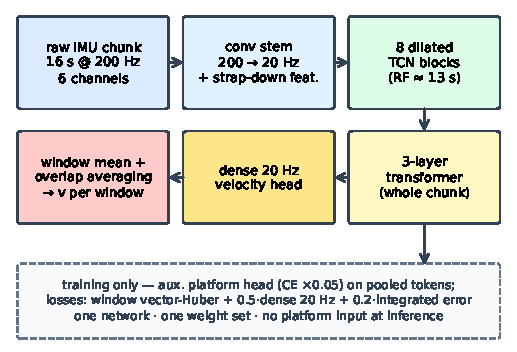
\includegraphics[width=\linewidth]{figures/pipeline.pdf}
    \caption{Overview of the method. One network, one weight set; the auxiliary platform head is discarded at inference.}
    \label{fig:method_overview}
\end{figure}

\subsection{Data Processing}
Windows are used exactly as defined ($k{\cdot}200$ to $(k{+}1){\cdot}200$); trajectories are kept whole in memory
and training samples are random 16-window chunks (edge-padded and loss-masked when a trajectory is shorter).
Dense 20\,Hz targets are the 10-sample means of \texttt{vel\_body}. Augmentation, all on device and per chunk:
\textbf{sensor re-mount rotation} (uniform random axis, angle $U(0,15^\circ)$; $U(0,45^\circ)$ for drone chunks)
applied identically to accelerometer, gyroscope and target velocity, i.e.\ an exact re-mounting;
\textbf{time dilation} by $s\sim\log U(1/1.3,1.3)$: the chunk is resampled, $v\!\to\!sv$, $\omega\!\to\!s\omega$
and the dynamic acceleration $\to s^{2}$ while the gravity component (from the training quaternion) is kept;
accelerometer scale $1{+}\mathcal N(0,0.02)$, bias $\mathcal N(0,0.15\,\mathrm{m/s^2})$, gyroscope scale
$1{+}\mathcal N(0,0.02)$, bias $\mathcal N(0,0.02\,\mathrm{rad/s})$, white noise $\sigma{=}0.05$ / $0.004$.
No filtering, resampling or calibration is applied at inference.

\subsection{Training Data}
Only the official challenge data was used (Table~\ref{tab:datasets}). Model selection used the released
\texttt{train}/\texttt{val} split (395/80 trajectories); the final model was refit on train+val with the schedule
fixed by the val experiments. No external data, synthetic data, pretrained checkpoints or pseudo-labels.
Test information was never used: test files were read only by the inference script.
\begin{table}[htbp]
    \centering\footnotesize
    \caption{Datasets used for model development and training.}
    \begin{tabular}{p{2.3cm} p{1.6cm} p{3.4cm}}
        \toprule Dataset & Type & Usage \\ \midrule
        Challenge \texttt{train} & Official & Training of all selection runs \\
        Challenge \texttt{val} & Official & Model/recipe selection (never trained on in selection runs); folded into the final refit \\
        \bottomrule
    \end{tabular}
    \label{tab:datasets}
\end{table}

\subsection{Training and Optimization}
Loss: $L = L_{\mathrm{win}} + 0.5\,L_{\mathrm{dense}} + 0.2\,L_{\mathrm{drift}} + 0.05\,L_{\mathrm{plat}}$, where
$L_{\mathrm{win}}$ is a vector Huber ($\beta{=}0.25$\,m/s) on the per-window mean velocity, $L_{\mathrm{dense}}$
the same on the 20\,Hz output, $L_{\mathrm{drift}}=\frac1T\sum_t \lVert\sum_{k\le t}(\hat v_k - v_k)\rVert/\sqrt t$
an integrated body-frame error mirroring ATE$_{20}$'s sensitivity to correlated bias, and $L_{\mathrm{plat}}$ the
auxiliary cross-entropy. AdamW ($\beta{=}0.9/0.99$, weight decay 0.02), OneCycle (peak $1.5{\times}10^{-3}$,
8\,\% warm-up), batch 64 chunks, 250 steps/epoch, gradient clipping 2.0, EMA of the weights (0.998) and a uniform
average of the EMA weights over the last 20 epochs (SWA). Sampling: platform uniform, then trajectory uniform
within the platform. Selection runs: 60 epochs; final refit: 160 epochs, single stage, no curriculum, no
fine-tuning, no platform-specific specialization. The final checkpoint is the SWA weights at the end of the fixed
schedule -- no early stopping is possible because val is inside its training set. Hardware: Apple M5 laptop GPU for
all selection runs (1.9--3\,min/epoch); the ranked checkpoint was trained by a Kaggle script kernel on a Kaggle
GPU in 3.6\,h.

\subsection{Inference}
For each test trajectory, 16-window chunks slide with a stride of 2 windows; each chunk is run once; per-window
outputs are averaged across overlapping chunks with a raised-cosine weight (+0.05 floor) so a window is trusted most
from the chunk in which it is central. Trajectories shorter than 16 windows are edge-padded and the padding
discarded. Trajectories are processed independently. No TTA, no ensembling, no scaling, smoothing or clipping, no
test-time adaptation. Inference uses past and future context of the same trajectory (offline).

\subsection{Model Complexity and Runtime}
Table~\ref{tab:runtime}. The method is offline (bidirectional); a causal variant would need a different design.
\begin{table}[htbp]
    \centering\footnotesize
    \caption{Model complexity and runtime statistics.}
    \begin{tabular}{p{2.6cm} p{5.2cm}}
        \toprule Property & Value \\ \midrule
        Number of parameters & 3.9\,M (second entry: 1.8\,M) \\
        Training hardware & Kaggle GPU (ranked run); Apple M5 laptop GPU (selection runs) \\
        Training time & 3.6\,h (160 epochs $\times$ 250 steps $\times$ 64 chunks) \\
        Inference hardware & any single GPU ($<$2\,GB VRAM) or CPU \\
        Inference speed (Hz) & $\approx$500 windows/s on a laptop GPU (whole test set $<$1\,min); CPU: tens of minutes \\
        Peak memory & $<$2\,GB GPU; $\approx$3\,GB RAM \\
        \bottomrule
    \end{tabular}
    \label{tab:runtime}
\end{table}

%%%%%%%%%%%%%%%%%%%%%%%%%%%%%%%%%%%%%%%%%%%%%%%%%%%%%%%%%%%%%%%%%%%%%%%%%%%%%%%%
\section{Development Experiments}
\label{sec:devexp}
All numbers below are val scores (organizers' scorer, 80 held-out trajectories) of models trained on
\texttt{train} only, unless stated. Fig.~\ref{fig:val_curves} shows the curves.

\textbf{Context is the largest gain.} A per-window 1D ResNet in the style of the public starter kernel reaches
$\approx$0.30; our first 16\,s-context model (width 128, 30 epochs) reached \textbf{0.2247}. A 32\,s context with
a wider trunk was \emph{worse} at equal epochs (0.2293), so 16\,s was kept.

\textbf{Longer schedules.} The same recipe for 60 instead of 30 epochs: 0.2233$\to$\textbf{0.2030}
(drone-B AVE 0.328$\to$0.271, car 0.129$\to$0.117, human 0.085$\to$0.073). On the public leaderboard the
train+val refits went 0.3625 (30 ep) $\to$ 0.3466 (60) $\to$ 0.2975 (100) $\to$ 0.2870 (160); 240 epochs gave no
further gain (0.2897).

\textbf{Metric-shaped sampling.} Sampling trajectories uniformly within a platform instead of proportionally to
length: 0.2030$\to$\textbf{0.1982}, with the largest effect on the short, hard drone trajectories -- the metric
averages per trajectory, so short trajectories count as much as long ones.

\textbf{Model scale.} Width 192 with a 3-layer transformer instead of 128/2: 0.2030$\to$0.1987 on val, but the
corresponding train+val refits scored 0.2893 and 0.2861--0.2876 publicly versus 0.2870 for the narrow model,
i.e.\ within leaderboard noise (Sec.~\ref{sec:selection}). Scale helped every platform slightly and hurt none.

\textbf{Drone-targeted augmentation.} Rotations up to 45$^\circ$ for drone chunks, $\times$4 oversampling of the
racing-drone source and time dilation: 0.2247$\to$0.2233 overall but \emph{no change} on the racing-drone
trajectories (AVE 0.674$\to$0.676). Increasing the drone sampling share to 40\,\% (0.2013) and vibration-amplitude
augmentation (0.2065) were both worse than uniform sampling (0.1982).

\textbf{Things that did not work} (cost in parentheses): raw strap-down features alone gave no measurable gain --
16\,s integration drifts by 5--20\,m/s under uncompensated gyro bias, so the network's implicit short-horizon
integration is already better (2\,h); a learned per-chunk IMU$\leftrightarrow$ground-truth \emph{time-shift head},
supervised by measured offsets, predicted the offsets of unseen recordings well ($-66$/$-48$\,ms predicted vs
$-40$/$-70$ measured) but did not improve the score (2\,h); rotation TTA (0.2246 vs 0.2247), 3-window smoothing
(ATE worse on every platform), denser overlap (identical), a bidirectional GRU context module (same accuracy,
3$\times$ slower on our hardware). Prediction averaging of 2--4 runs improved val to 0.2171 and public to 0.354
(from 0.363) but is not a single weight set and was not used for any ranked entry.

\begin{figure}[htbp]
    \centering
    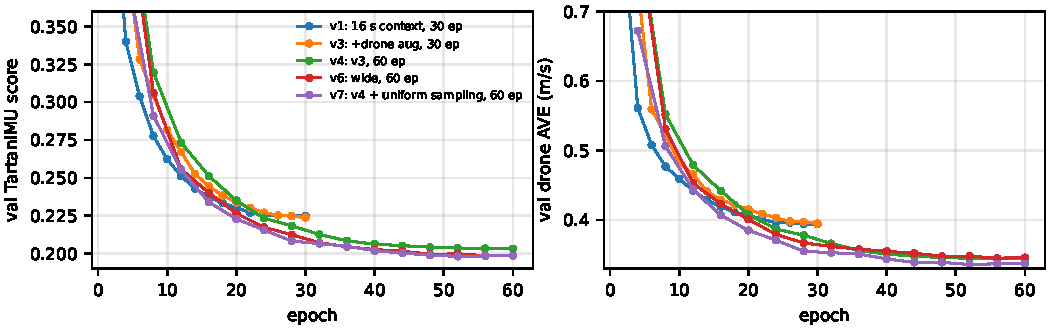
\includegraphics[width=\linewidth]{figures/val_curves.pdf}
    \caption{Validation score and drone AVE during training for the main selection runs (train only, scored on the
    held-out val split every 2--4 epochs).}
    \label{fig:val_curves}
\end{figure}

%%%%%%%%%%%%%%%%%%%%%%%%%%%%%%%%%%%%%%%%%%%%%%%%%%%%%%%%%%%%%%%%%%%%%%%%%%%%%%%%
\section{Experiments}
\subsection{Official Challenge Performance}
Tables~\ref{tab:overall_results}--\ref{tab:sequence_results} were produced by the official scoring service for the
CSV of our ranked Kaggle submission 56402554, \texttt{md5 = \textbf{fd12d4f25d7b52d44aaa4e4a14534378}}
(scored under the team's pre-rename Kaggle name ``Md.\ Hamid Hosen''; the team was renamed Hack2Publish on 21 Sept.
and the service's whitelist had not yet refreshed). Full-test score \textbf{0.21903}; public leaderboard 0.28609 (rank
9 of 108 at close). The second selected entry (56332266, md5 \texttt{97a6e86dba7dfc19929e050bef5857b0}) scores 0.22189
on the same service (AVE 0.181, ATE$_{20}$ 0.581). The drone term carries 64\,\% of our score (Table~\ref{tab:platform_results}):
AVE is 0.05--0.07\,m/s on car, human and dog but 0.52\,m/s on drone, and ATE$_{20}$ 0.36--0.49\,m versus 1.04\,m.
\begin{table}[htbp]
    \centering\footnotesize
    \caption{Overall challenge performance (official scoring service, full 89-sequence test set). The TartanIMU Score is
    $0.6\,\mathrm{AVE}/0.7356 + 0.4\,\mathrm{ATE}_{20}/3.1160$, dimensionless, \emph{lower is better} (all-zero = 1.000).
    \textbf{RTE does not enter the ranking}; it is defined in the caption of Table~\ref{tab:sequence_results}.
    Baseline numbers are the organizers' published full-test values.}
    \setlength{\tabcolsep}{3.5pt}
    \begin{tabular}{lcccc}
        \toprule Method & Score $\downarrow$ & ATE$_{20}$ $\downarrow$ & AVE $\downarrow$ & RTE $\downarrow$ \\ \midrule
        TartanIMU Baseline & 0.538 & 1.261 & 0.461 & -- \\
        Ours (Hack2Publish) & 0.2190 & 0.563 & 0.180 & 0.868 \\
        \bottomrule
    \end{tabular}
    \label{tab:overall_results}
\end{table}

\begin{table}[htbp]
    \centering\footnotesize
    \caption{Performance by platform (official scoring service). RTE is defined in the caption of Table~\ref{tab:sequence_results}.}
    \begin{tabular}{lccc}
        \toprule Platform & ATE$_{20}$ $\downarrow$ & AVE $\downarrow$ & RTE $\downarrow$ \\ \midrule
        Wheeled / Car & 0.369 & 0.071 & 0.323 \\
        Handheld / Human & 0.490 & 0.053 & 0.270 \\
        Legged / Quadruped & 0.358 & 0.074 & 0.353 \\
        Aerial / Drone & 1.037 & 0.522 & 2.528 \\
        \midrule Average & 0.563 & 0.180 & 0.868 \\
        \bottomrule
    \end{tabular}
    \label{tab:platform_results}
\end{table}


\subsection{Per-Sequence Results}
The error is concentrated, not spread (Table~\ref{tab:sequence_results}): a minority of drone sequences -- those of
the racing-drone source (short, 3--7\,m/s, two IMUs per flight, Sec.~\ref{sec:data}) -- have AVE several times that of
any other sequence and account for most of the drone term, which itself is 64\,\% of the score. Within the
other platforms the per-sequence errors are homogeneous (car/dog/human AVE 0.07--0.13\,m/s in val); the slow
hovering drone sequences have an AVE equal to the standard deviation of their own ground-truth velocity, i.e.\ the
model predicts the mean and cannot resolve sub-0.2\,m/s hover drift from the IMU.

\subsection{Ablation Studies}
Section~\ref{sec:devexp} is our ablation record; in decreasing order of effect on val: trajectory context
($-$0.08), schedule length ($-$0.02), uniform trajectory sampling ($-$0.005), model scale ($-$0.004), drone
augmentation ($-$0.001), physics features / time-shift head / TTA / smoothing (0 or negative).

\subsection{Generalization Analysis}
\label{sec:data}
Val (disjoint trajectories) tracks the test set closely: val 0.198 vs 0.219 on the full test set, while the public
split is much harder (0.286); the organizers' baseline shows the same pattern (0.538 full test vs 0.637 public). The
difference is explained by the drone split. Fig.~\ref{fig:scatter} shows the per-trajectory val error of our recipe: car, dog and human errors are
0.07--0.13\,m/s regardless of speed; drone-B (the second drone source) errors are 0.15--0.4\,m/s and, remarkably,
\emph{lower} at 3--4\,m/s than when hovering; drone-A (racing drone) errors are 0.45--1.0\,m/s at every speed.

Two data findings explain this, both measured on the released train/val files.
\emph{(1)~Frame convention of drone-B.} Its gyroscope $z$ axis is inverted relative to the quaternion/velocity
body frame (ground-truth yaw rate $= -\omega_z$, $R^2{=}0.97$), and its accelerometer dynamics match the
ground-truth specific force under no axis relabelling ($R^2{<}0$ at 2\,Hz, unconstrained fits give axis gains of
0.6--2.1), whereas the other three platforms and drone-A have identity conventions with $R^2$ 0.97--0.99. The
network still learns drone-B well because the source is trivially identifiable from the signal (high-frequency
accelerometer content differs by 10$\times$), but the physics it learns there does not transfer to drone-A, which
has only $\approx$30\,min of data.
\emph{(2)~Racing-drone recordings.} Every fast flight appears twice, recorded by two IMUs (one level, one pitched
$\approx$45$^\circ$, e.g.\ \texttt{drone\_val\_0005/0006}). Their IMU streams are offset from the ground truth by
\emph{different} amounts ($\approx-10$\,ms for one IMU type, $-40\ldots-70$\,ms for the other, measured by
cross-correlating $|\omega|$ with the quaternion-derived rate), and after time alignment and the best-fit
rotation the two recordings' velocity targets still disagree by 0.15--0.9\,m/s ($\approx$5$^\circ$ of mount
inconsistency at 4--7\,m/s). This is a floor on that source that no IMU-only model can pass, and about a quarter of
the test drone trajectories are of this type. Several dog trajectories also have offsets of 40--150\,ms.
We found no evidence of negative transfer between platforms: every platform improved with every improvement of
the shared recipe, and removing a platform never helped another.

\begin{figure}[htbp]
    \centering
    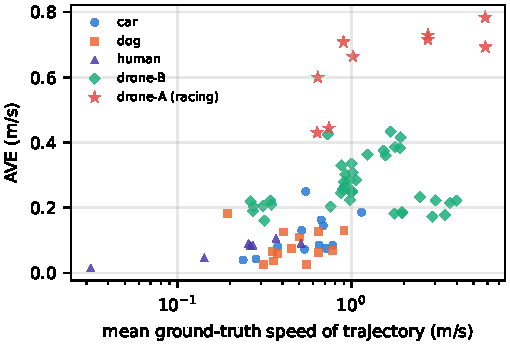
\includegraphics[width=0.9\linewidth]{figures/val_scatter.pdf}
    \caption{Per-trajectory val AVE of the final recipe (train-only run) against mean speed. The racing-drone
    source is an outlier at every speed; the slowest drone-B sequences sit at the floor set by hover drift.}
    \label{fig:scatter}
\end{figure}

\subsection{Failure-Mode Analysis}
(i)~Racing-drone flights: errors of 0.5--1\,m/s that are bias-like per recording, consistent with the timing and
mount inconsistencies above. (ii)~Slow hover: velocity variations of $\pm$0.15\,m/s at 0.1\,Hz produce
$\approx$0.1\,m/s$^2$ of acceleration under 4--6\,m/s$^2$ of vibration -- unobservable. (iii)~Fast cars ($>$3\,m/s,
25 windows in val) have errors of 3--4\,m/s: this regime does not exist in the training data. Unresolved: a
principled way to make the drone-B convention consistent with the rest of the data (it is not a fixed axis
relabelling), and any use of the two-IMU redundancy.

%%%%%%%%%%%%%%%%%%%%%%%%%%%%%%%%%%%%%%%%%%%%%%%%%%%%%%%%%%%%%%%%%%%%%%%%%%%%%%%%
\section{Insights and Lessons Learned}
\label{sec:insights}
\textbf{A single universal model is feasible for the part of the problem that is observable.} One 3.9\,M-parameter
network with no platform input reaches 0.07--0.13\,m/s AVE on car, dog and human and $\approx$0.27\,m/s on ordinary
drone flight, and every change that helped one platform helped the others. The embodiment is inferred implicitly
and reliably; specialization was never needed. \textbf{The bottleneck is data quality and observability, not the
model.} Our largest remaining error comes from a source whose labels are internally inconsistent at the level of
tens of milliseconds and a few degrees; more capacity, more epochs and more augmentation all left it untouched,
while everything else kept improving. \textbf{Context transfers; conventions do not.} Reading whole trajectories,
metric-shaped sampling and physically exact augmentation are sensor- and platform-agnostic and should transfer to
other IMUs and vehicles; anything learned about a specific source's axis convention or timing offset will not.
\textbf{Per hour of data, slow-and-clean beats fast-and-noisy}: 30\,min of racing-drone data contributed almost
nothing to generalization, while the drone-B hours drove the drone-B error down steadily. \textbf{Evaluation.} With
$\sim$45 drone test trajectories averaged per trajectory, a public split is dominated by a few short racing flights;
we measured $\pm$0.01--0.02 leaderboard differences between identical recipes. Promising directions: physics-informed
architectures that estimate bias, gravity and time offset explicitly with uncertainty; self-supervised consistency
between the two IMUs of the same flight; and datasets with verified time synchronization.

\subsection{Feedback to the Organizers}
The rules, metric and starter kit were unusually clear, and the exact scorer in the kit made local validation
trustworthy (our val floor 0.013 and all-zero 1.015 matched the published references). What cost us the most time
was discovering the data issues of Sec.~\ref{sec:data} ourselves; documenting per-source conventions, IMU types and
synchronization quality (or fixing the drone-B gyro sign and the racing-drone offsets) would let teams work on the
model instead. The metric behaved as documented, but the per-trajectory averaging makes short racing-drone clips
worth as much as 30-minute car drives, so the public leaderboard is noisy; averaging per window within a platform, or
a larger public split, would reduce it. The second-IMU duplicates of the same flights should be either merged or
declared. For the next edition, causal/online evaluation and a held-out platform would measure generalization more
directly than a platform-blind test set whose sources are identifiable from the signal.

%%%%%%%%%%%%%%%%%%%%%%%%%%%%%%%%%%%%%%%%%%%%%%%%%%%%%%%%%%%%%%%%%%%%%%%%%%%%%%%%
\section{Conclusion}
A trajectory-context network trained with a metric-shaped sampler and physically exact augmentation gives a single
unified inertial velocity estimator that is accurate on three of the four platforms and on ordinary drone flight,
reaching 0.219 on the full test set (0.286 on the harder public split, from our own starting point of 0.553) with one
weight set and no post-processing. The remaining error is dominated by one drone source whose ground truth is internally inconsistent;
closing it requires better data, or models that estimate synchronization and mounting explicitly.

\section*{ACKNOWLEDGMENT}
We thank the CMU AirLab organizers for the dataset, the exact scorer and the scoring service, and Kaggle and Google
Colab for compute. The AI assistant Claude (Anthropic) was used for code development and analysis under the
authors' direction.

%%%%%%%%%%%%%%%%%%%%%%%%%%%%%%%%%%%%%%%%%%%%%%%%%%%%%%%%%%%%%%%%%%%%%%%%%%%%%%%%
\section*{APPENDIX}
\subsection{Per-Sequence Results (Full Table)}
\begin{table*}[htbp]
    \centering\footnotesize
    \caption{Per-sequence challenge results over the 89 test sequences (official per-sequence scoring service; submission md5
    \texttt{fd12d4f25d7b52d44aaa4e4a14534378}). \textbf{RTE} (Relative Trajectory Error, m) follows Sturm \emph{et al.}~\cite{sturm2012rgbd}:
    over sliding windows of $\Delta t = 5$\,s, the RMSE of the difference between predicted and ground-truth relative displacement,
    $\mathrm{RTE} = \sqrt{\frac{1}{n}\sum_i \lVert (\hat{\mathbf{p}}_{i+\Delta t} - \hat{\mathbf{p}}_i) - (\mathbf{p}_{i+\Delta t} - \mathbf{p}_i) \rVert^2}$.
    Sequence ids follow the scoring service's ordering.}
    \label{tab:sequence_results}
    \setlength{\tabcolsep}{4pt}
    \begin{tabular}{cccc @{\hspace{2em}} cccc @{\hspace{2em}} cccc}
        \toprule
        Seq. & ATE$_{20}$ & AVE & RTE & Seq. & ATE$_{20}$ & AVE & RTE & Seq. & ATE$_{20}$ & AVE & RTE \\ \midrule
        1 & 0.830 & 0.337 & 1.873 & 31 & 0.703 & 0.298 & 1.605 & 61 & 0.906 & 0.360 & 1.158 \\
        2 & 0.498 & 0.351 & 1.181 & 32 & 0.319 & 0.084 & 0.246 & 62 & 0.073 & 0.020 & 0.061 \\
        3 & 0.535 & 0.205 & 0.765 & 33 & 0.210 & 0.051 & 0.207 & 63 & 0.455 & 0.070 & 0.327 \\
        4 & 0.498 & 0.308 & 0.903 & 34 & 1.581 & 0.366 & 1.800 & 64 & 0.404 & 0.059 & 0.268 \\
        5 & 0.905 & 0.405 & 1.835 & 35 & 1.056 & 0.413 & 1.659 & 65 & 0.106 & 0.038 & 0.130 \\
        6 & 0.674 & 0.089 & 0.763 & 36 & 1.016 & 0.325 & 1.878 & 66 & 2.153 & 0.226 & 1.577 \\
        7 & 1.116 & 0.344 & 1.508 & 37 & 2.555 & 2.108 & 11.718 & 67 & 0.113 & 0.032 & 0.143 \\
        8 & 0.468 & 0.039 & 0.208 & 38 & 2.152 & 1.807 & 8.917 & 68 & 0.526 & 0.048 & 0.222 \\
        9 & 0.640 & 0.278 & 0.972 & 39 & 0.644 & 0.256 & 0.977 & 69 & 0.686 & 0.084 & 0.440 \\
        10 & 0.771 & 0.086 & 0.693 & 40 & 0.784 & 0.318 & 1.853 & 70 & 0.503 & 0.073 & 0.330 \\
        11 & 1.024 & 0.658 & 2.017 & 41 & 1.081 & 0.327 & 2.140 & 71 & 0.196 & 0.060 & 0.192 \\
        12 & 0.307 & 0.154 & 0.672 & 42 & 0.493 & 0.088 & 0.483 & 72 & 0.851 & 0.452 & 1.437 \\
        13 & 0.300 & 0.044 & 0.262 & 43 & 0.920 & 0.286 & 1.115 & 73 & 0.807 & 0.131 & 0.767 \\
        14 & 0.564 & 0.383 & 1.228 & 44 & 0.212 & 0.051 & 0.315 & 74 & 0.595 & 0.310 & 1.006 \\
        15 & 1.021 & 0.073 & 0.409 & 45 & 0.083 & 0.053 & 0.126 & 75 & 0.548 & 0.393 & 1.216 \\
        16 & 0.127 & 0.034 & 0.224 & 46 & 0.258 & 0.059 & 0.241 & 76 & 0.399 & 0.097 & 0.423 \\
        17 & 1.136 & 0.559 & 2.669 & 47 & 0.840 & 0.387 & 1.063 & 77 & 1.166 & 0.567 & 2.337 \\
        18 & 1.360 & 0.565 & 2.554 & 48 & 0.211 & 0.015 & 0.101 & 78 & 0.197 & 0.029 & 0.098 \\
        19 & 0.521 & 0.294 & 1.308 & 49 & 0.798 & 0.255 & 1.343 & 79 & 0.817 & 0.261 & 1.419 \\
        20 & 0.140 & 0.053 & 0.370 & 50 & 0.669 & 0.210 & 1.117 & 80 & 0.448 & 0.174 & 0.910 \\
        21 & 0.706 & 0.209 & 1.133 & 51 & 0.080 & 0.037 & 0.097 & 81 & 0.645 & 0.116 & 0.474 \\
        22 & 0.573 & 0.391 & 1.197 & 52 & 0.258 & 0.070 & 0.359 & 82 & 2.896 & 0.389 & 2.533 \\
        23 & 1.027 & 0.241 & 1.984 & 53 & 0.394 & 0.279 & 0.513 & 83 & 0.449 & 0.074 & 0.372 \\
        24 & 0.392 & 0.043 & 0.193 & 54 & 0.222 & 0.070 & 0.260 & 84 & 0.477 & 0.057 & 0.321 \\
        25 & 0.105 & 0.029 & 0.109 & 55 & 0.269 & 0.144 & 0.665 & 85 & 0.074 & 0.032 & 0.097 \\
        26 & 0.596 & 0.086 & 0.353 & 56 & 3.406 & 2.896 & 15.349 & 86 & 0.305 & 0.027 & 0.148 \\
        27 & 0.476 & 0.060 & 0.290 & 57 & 0.922 & 0.356 & 2.145 & 87 & 0.414 & 0.173 & 0.657 \\
        28 & 0.566 & 0.256 & 1.271 & 58 & 0.219 & 0.050 & 0.250 & 88 & 1.028 & 0.294 & 2.012 \\
        29 & 3.661 & 2.886 & 16.039 & 59 & 0.361 & 0.074 & 0.385 & 89 & 0.148 & 0.028 & 0.091 \\
        30 & 1.136 & 0.548 & 2.608 & 60 & 0.156 & 0.066 & 0.214 &  & & &  \\
        \bottomrule
    \end{tabular}
\end{table*}


\subsection{Reproducibility and Submission Artifacts}
\label{sec:selection}
\begin{sloppypar}\raggedright
Kaggle team \textbf{Hack2Publish}. Ranked submission \textbf{56402554} (\texttt{submission\_final\_kaggle\_w\_uni.csv},
2026-09-20 17:34 UTC, md5 \texttt{fd12d4f25d7b52d44aaa4e4a14534378}, public 0.28609). Second selected entry
\textbf{56332266} (\texttt{submission\_final\_v4\_160.csv}, md5 \texttt{97a6e86dba7dfc19929e050bef5857b0},
public 0.28696): the width-128 / 2-layer variant trained on an Apple M5 with length-weighted sampling.
Code: the GitHub repository below (training commit \texttt{a9a5384}; the Kaggle kernel script that trained the ranked checkpoint is in
\texttt{kaggle\_kernel/}). Checkpoints: the Hugging Face repository below -- \texttt{model.pt}
(SHA-256 \texttt{69764745d0589eba846d571b364aa3d3\allowbreak 3fe6a25be5e516879339b3231ceeb9b1}) and
\texttt{model\_secondary\_final\_v4\_160.pt} (\texttt{f1eb2086\ldots}), with \texttt{infer.py}, \texttt{model.py},
pinned \texttt{requirements.txt} (torch 2.14.0, numpy 2.5.2, pandas 3.0.5) and \texttt{SHA256SUMS}; the exact argparse
configuration is stored inside each checkpoint and in \texttt{configs/}. Seed 0; every reported score is a single run.
Run-to-run spread: the identical recipe trained on two different GPUs scored 0.2870 and 0.3052 publicly, and the
ranked recipe 0.2861 (Kaggle GPU) vs 0.2876 (laptop). Inference reproduces the submitted CSV to $\le$0.005\,m/s per
window across devices (TF32 disabled).

\noindent\textbf{Compliance declaration.}
\begin{enumerate}
    \item \textbf{Yes.} All predictions come from a single model with one shared set of weights.
    \item \textbf{No} platform classification, routing or specialization at inference. An auxiliary platform head
    exists in the training graph only; its output is never computed at inference and nothing depends on it.
    \item \textbf{No} model ensembling and \textbf{no} test-time augmentation. Weight averaging within a single run
    only: EMA of the weights during training and a uniform average of the EMA weights over the last 20 epochs.
    \item Test data was read only by the inference script. All architecture and hyper-parameter choices were made
    on the released \texttt{val} split with the organizers' scorer; the final model is a fixed-schedule refit on
    train+val with no checkpoint selection. Among the finished refits, the two Kaggle entries were chosen by
    val-validated recipe first and public score second; no training or post-processing was tuned against the
    leaderboard.
    \item The development-time system and the submitted system are identical. The only differences between the
    ranked and the second entry are the trunk width / transformer depth and the sampling weights, as stated above.
\end{enumerate}
\end{sloppypar}

\subsection{Final Predictions}
The ranked CSV (30,644 rows, columns \texttt{window\_id,vx,vy,vz}, md5 above) is attached to the Submission Form and
is regenerated bit-exactly on the training device from the Hugging Face repository by\\
\texttt{python infer.py --traj\_dir test \allowbreak --windows index/test\_windows.csv \allowbreak --out submission.csv}. No post-processing is applied after
the network output beyond the overlap averaging described in Sec.~II-E; there are no missing or degenerate windows.

\subsection{Model and Inference Code}
Weights, inference entry point, configuration and environment (Hugging Face):\\
\hfrepo\\
Training code, analysis scripts and this report's sources (GitHub):\\
\ghrepo

\begin{thebibliography}{99}
\bibitem{tartanimu}
S.~Zhao, S.~Zhou, R.~Blanchard, Y.~Qiu, W.~Wang, and S.~Scherer, ``Tartan IMU: A Light Foundation Model for Inertial
Positioning in Robotics,'' in \emph{Proc.\ IEEE/CVF CVPR}, 2025, pp.~22520--22529.
\bibitem{sturm2012rgbd}
J.~Sturm, N.~Engelhard, F.~Endres, W.~Burgard, and D.~Cremers, ``A Benchmark for the Evaluation of RGB-D SLAM
Systems,'' in \emph{Proc.\ IEEE/RSJ IROS}, 2012, pp.~573--580.
\bibitem{ronin}
S.~Herath, H.~Yan, and Y.~Furukawa, ``RoNIN: Robust Neural Inertial Navigation in the Wild,'' in \emph{Proc.\ IEEE
ICRA}, 2020.
\bibitem{tlio}
W.~Liu, D.~Caruso, E.~Ilg, J.~Dong, A.~Angelova, and S.~Belongie, ``TLIO: Tight Learned Inertial Odometry,''
\emph{IEEE RA-L}, vol.~5, no.~4, 2020.
\end{thebibliography}
\end{document}
